\documentclass[final]{cmpreport}
\RequirePackage{natbib}
\usepackage[utf8]{inputenc}
\usepackage{pgfgantt}
\usepackage{algorithm}   % For math symbols
\usepackage[noend]{algpseudocode}
\setcitestyle{numbers}

\title{Project Portfolio - How can I check?}
\author{James Wright }
\date{October 2021}
\registration{100301701}
\ccode{CMP-6001Y}
\supervisor{Katharina Huber}
\summary{This will be a report detailing on how I designed an application for Students to check their answers to questions based on Linear Algebra and Calculus. It will detail my plans, the features of the application, methodology and then the results of the app. Further analysis will then conclude the success of the methodology.}
\begin{document}

			\begin{figure}[H]
		\caption{Report poster}
		\centering
		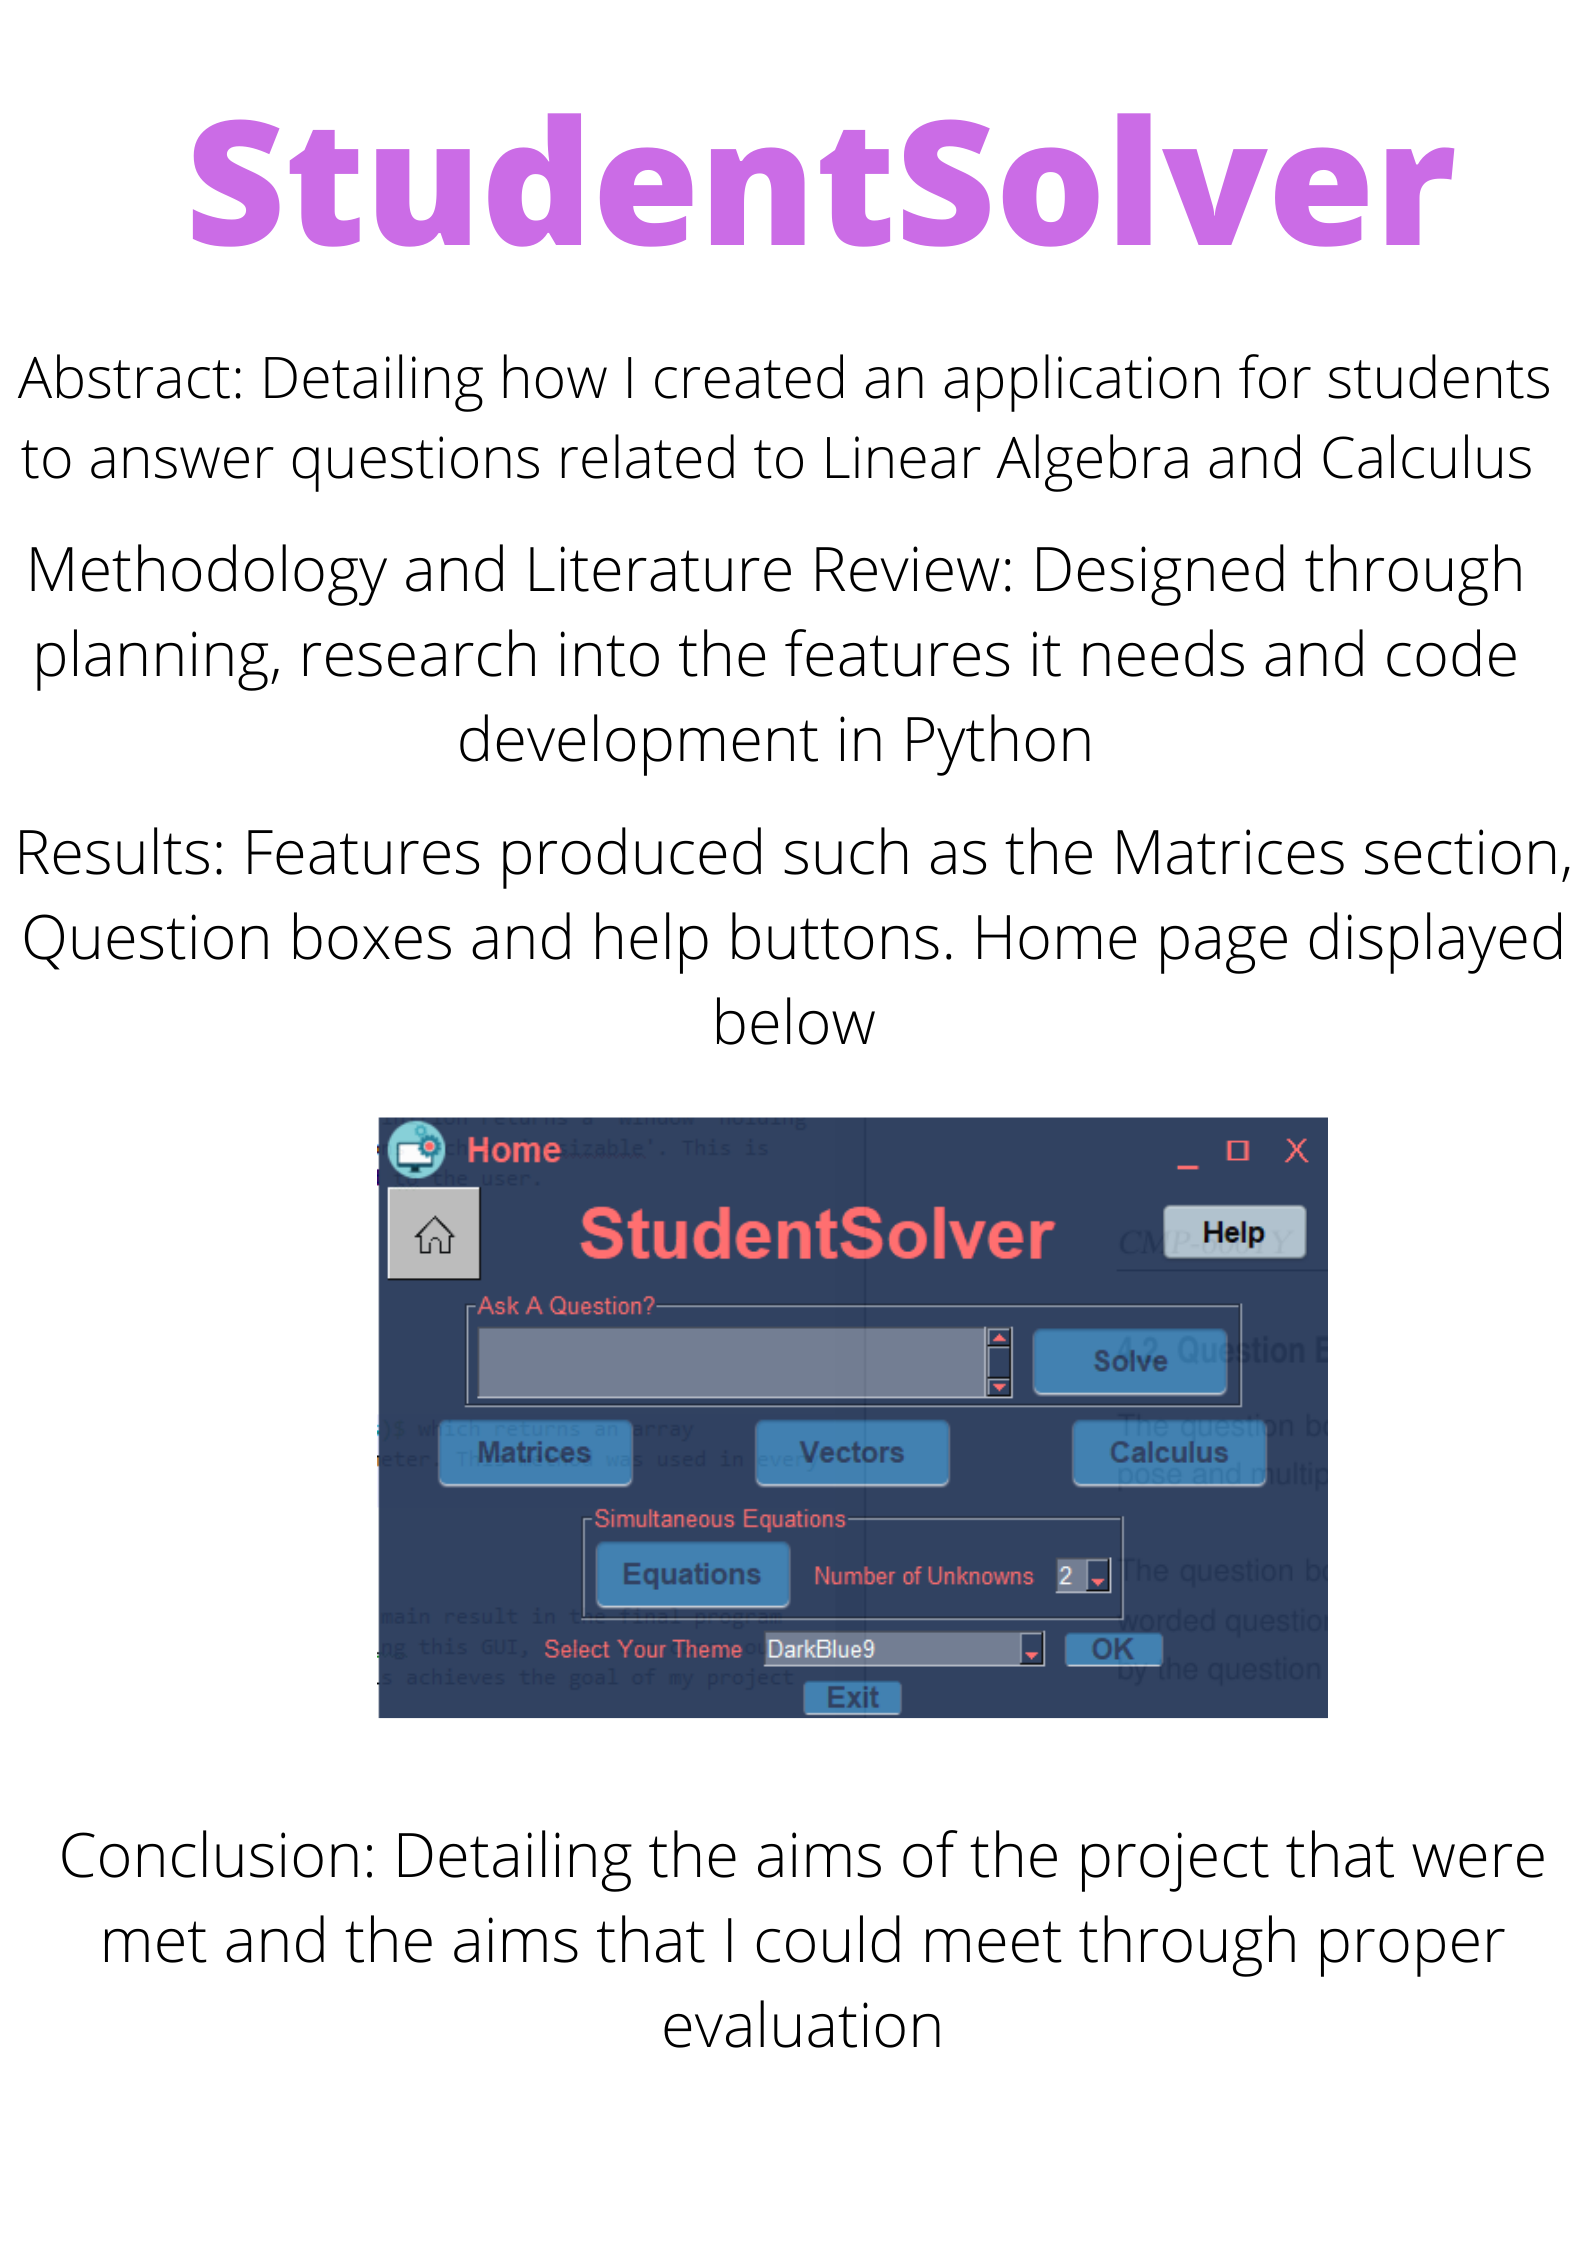
\includegraphics[scale=0.3]{poster.png}
		\label{fig:poster}
	\end{figure}
	\section{Introduction} \label{sec:intro}
	
	Questions such as "How can I check if my answers are correct?" are on the mind of many students preparing for their assessments. The main objective of this project is to develop a easy-to-use and simple desktop application that will allow students to address this question in mathematical terms. The application is to be delivered as an executable compatible on Windows computers, containing interactive features such as buttons and simple user input.\\
	\\The users of this application will be students studying A-Level Mathematics and/or Further Mathematics. I chose A-Level students as my target audience due to the complexity of the questions typically asked of them. This can make finding the solution time-consuming and prone to mistakes.  My application aims to combat this by offering detailed solutions for complex tasks, and reduce the time taken for students to find these solutions.\\
	\\The application must be usable, highly tested and open-source. Usability will be achieved by the ease of which a student can navigate around the application to be able to receive an answer from a mathematical question.\\
	\\To do this, the program will have categorised windows dedicated to specific topics. These topics will be consistent with those A-Level Mathematics students will be learning in their course. This program focuses on the Linear Algebra and Calculus categories of the course.\\
	\\Testing will be judged based on the number of lines the test files have covered in the application's code. It will also be judged through heavy user testing, ensuring the program is both usable and free from any errors. This should be done from the perspective of my intended audience. The results of testing are detailed in Section \ref{sec:test} of this report. \\
	\\The program must have a clear development structure, allowing other developers to use the application and carry out further improvements. This has been achieved through making the code open-source, meaning anyone online can download the application files and edit it themselves. Albeit they will have their own copy of the application.\\
	\\Conceptual challenges I faced in this project include what features the application will have, the mathematical topics it will cover, and how the program should 'look and feel'. The technical challenges I faced is the development of a GUI (Graphical User Interface) and programs to carry out mathematical operations. These challenges are overcome through research on both sites containing similar features, and documentation on Python libraries. \\
	\\Section \ref{sec:lit} aims to detail and answer any research questions. The methodology part of this paper(\ref{sec:method}) details how I achieved my objectives through development, planning and design. Then I have detailed the results of my methodology in Section \ref{sec:results}.\\
	\\My project notebook contains all personal notes and any updates I have made to planning. It also contains figures for pseudocode.
	

	\section{Literature Review} \label{sec:lit}
	
	As this is a digital application, I will be reviewing applications with similar goals shown in \ref{sec:intro}, and sites that use syntax formatting to input mathematical questions. The review will be based on it's usability for my target audience and it's features. I will also review sites that were used heavily for research that contributed to the class design and development.\\
	\\In sections \ref{sec:wolf} and \ref{sec:math}, the purpose of this review is to assess the features websites contain that answer mathematical questions. For \ref{sec:rev} and \ref{sec:fur}, sites named 'Further Maths Tutor' and 'Revision Maths' are reviewed for their education on the A-Level Curriculum for Mathematics, and the contribution of topics provided in the application. Finally, section \ref{sec:pysimple} will detail the extent to which the library named 'PySimpleGUI' is documented and it's effectiveness in aiding myself to create a graphical user interface.
	
	\subsection{Wolfram Alpha} \label{sec:wolf}
	Wolfram Alpha \cite{Wolfram-Alpha} is a website that allows you to input an equation and it will display you step-by-step solutions. The solutions is a feature I will be using in a similar manner to Wolfram Alpha. Figure \ref{fig:step} shows an example of quadratic expansion. The important details that makes the solutions easy to read is the simplification of the equation in step 2 to visually show the next step, which then shows each calculation done for the multiplication. Step 4,5 and 6 show each term being added individually and the final answer is clearly displayed in a blue box. \\
	\\My application will improve on that format by including wording to explain the step in a bit more detail. For example step 2 doesn't explain that it is multiplying each term twice in the brackets, meaning that someone who has little knowledge on expanding to polynomials may be confused as to the steps. It is very important that users understand the solutions as the whole point of the application is to educate.\\
	\begin{figure}[H]
		\caption{Step-by-step solution for expanding $(x+3)^2$ detailed in each box the page contains}
		\centering
		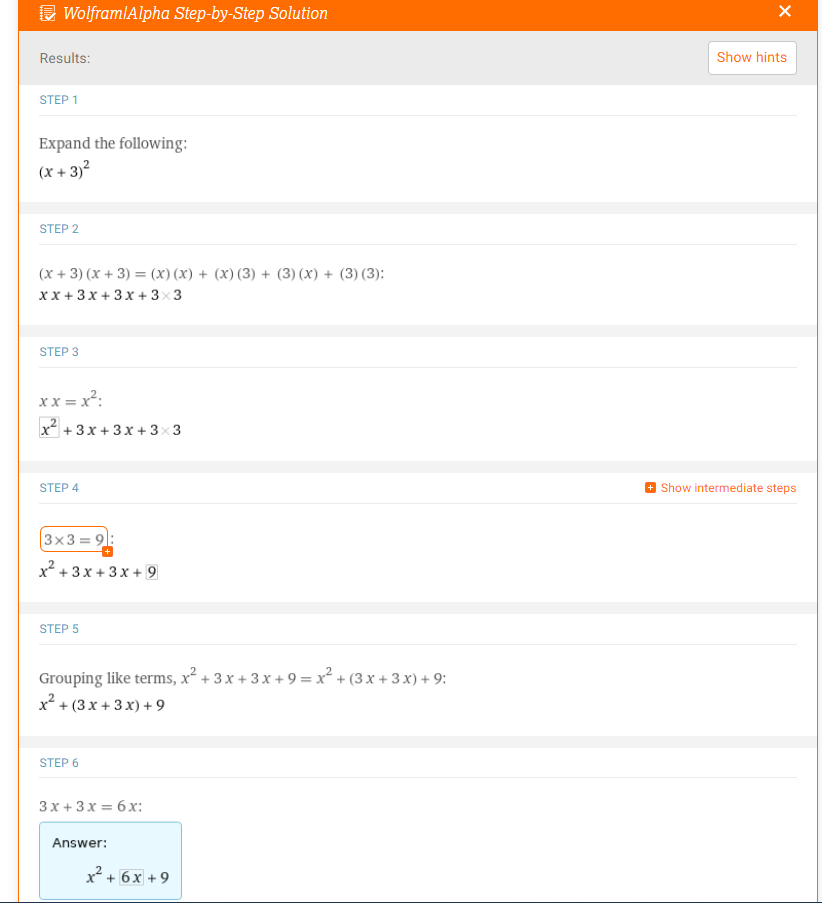
\includegraphics[height=110mm]{step.png}
		\label{fig:step}
	\end{figure}
	\begin{figure}[H]
		\caption{Use of syntax formatting in the input box at the top of the figure.}
		\centering
		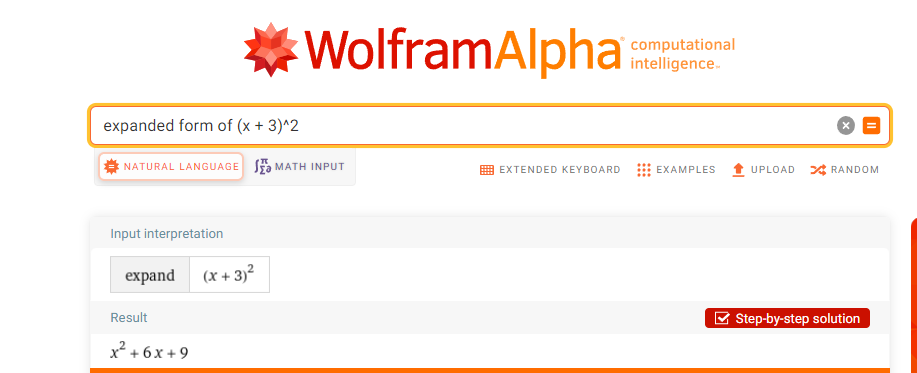
\includegraphics[scale=0.5]{step2.png}
	\end{figure}
	The site uses general syntax formatting that is easy-to-use. General syntax formatting means the standard of syntax used for equations worldwide. An example of the source's syntax formatting would be using "y''" to show a 2nd order differential for y ($\frac{d^2x}{dy^2} y$). \\
	\\Figure 2 shows the input for figure 1. The wording is used as a command but is very simple for the user and program to recognize. Then $(x+3)^2$ is shown by using a circumflex to display the brackets squared. These are examples of general syntax that I will also be using in my application as well.\\
	\\Wolfram Alpha also offers an API which can be used to query the site and show the same results. I have used this for my question box on the GUI as discussed in \ref{sec:question}\\
	\\Visual representations can be given as well. For example simply typing "rotate 30 degrees", will show the rotation matrix and display it visually on a graph.
	Computations of shapes are simply done by specifying parameters and the shape name. For example, "5,12,13 triangle" will display the properties of the triangle with sides of length 5,12 and 13.\\
	\\However, I had to go onto help pages and find these examples showing more advanced questions are a lot harder for the average user to input. This is why I will categorize my application to have pages dedicated to certain operations, with a clear input box for users to input a matrix or vector.\\
	\\In summary, features such as visual representations, syntax formatting and step-by-step solutions will be very similar as to how I plan to design my application. However, it is clear Wolfram Alpha is more aimed at scientific topics that involve statistics and graphing whereas my application is designed more to educate pure mathematics and calculus. I show this by having more detailed step-by-step solutions and making the application more usable to my target audience. Therefore, this source was very helpful in determining what features I want, such as a question box and step-by-step solutions. \\
	
	\subsection{Microsoft Math Solver} \label{sec:math}
	
	Microsoft Math Solver \cite{math} is also a website allowing you to input equations and get a resulting output. Figure \ref{fig:output} shows a very basic solution to $ 4 \sin (   \theta     )   \cos (   \theta     )   =  2 \sin (   \theta     )   $. The solution has no wording, no explanation as to how it was calculated and also has variables that are unexplained such as $n$. The figure also shows a visual representation as a graph which is a feature I plan to include in my application.\\
	\\Figure \ref{fig:topic} shows basic topics on the home page and uses categories of Algebra, Trigonometry and Calculus. The labelling of each topic is easy to understand for a Maths student. When clicking on a label, the options are displayed on another page. I have used this idea in my application, as opposed to having options underneath a category. This is because if more topics get added in, the window of the application can contain too much text and buttons, decreasing it's usability.\\
	\\As for the syntax input, the user has a choice to use general syntax or an on-screen keyboard as shown in Figure \ref{fig:calc}. The on-screen keyboard is categorized in order to decrease its size pn the page and hold more options overall. It uses a matrix, algebra, trigonometry and an calculus calculator. Although this will make inputting data easier, it is not something I plan on implementing unless the plan allows for spare time. This is because it is not needed for a very simple application, as each page should hold a predefined set of boxes to input data. The calculator can also be confusing to some users, for example upon attempting to input a matrix I struggled actually being able to create the closing bracket for the data. I do not want there to be any confusion for the user inputting their data as it would decrease usability. \\
	\begin{figure}[H]
		\caption{Answer output. Input box at top of page, with $\theta$ being equal to the input solution. Also a graph below of the function. }
		\centering
		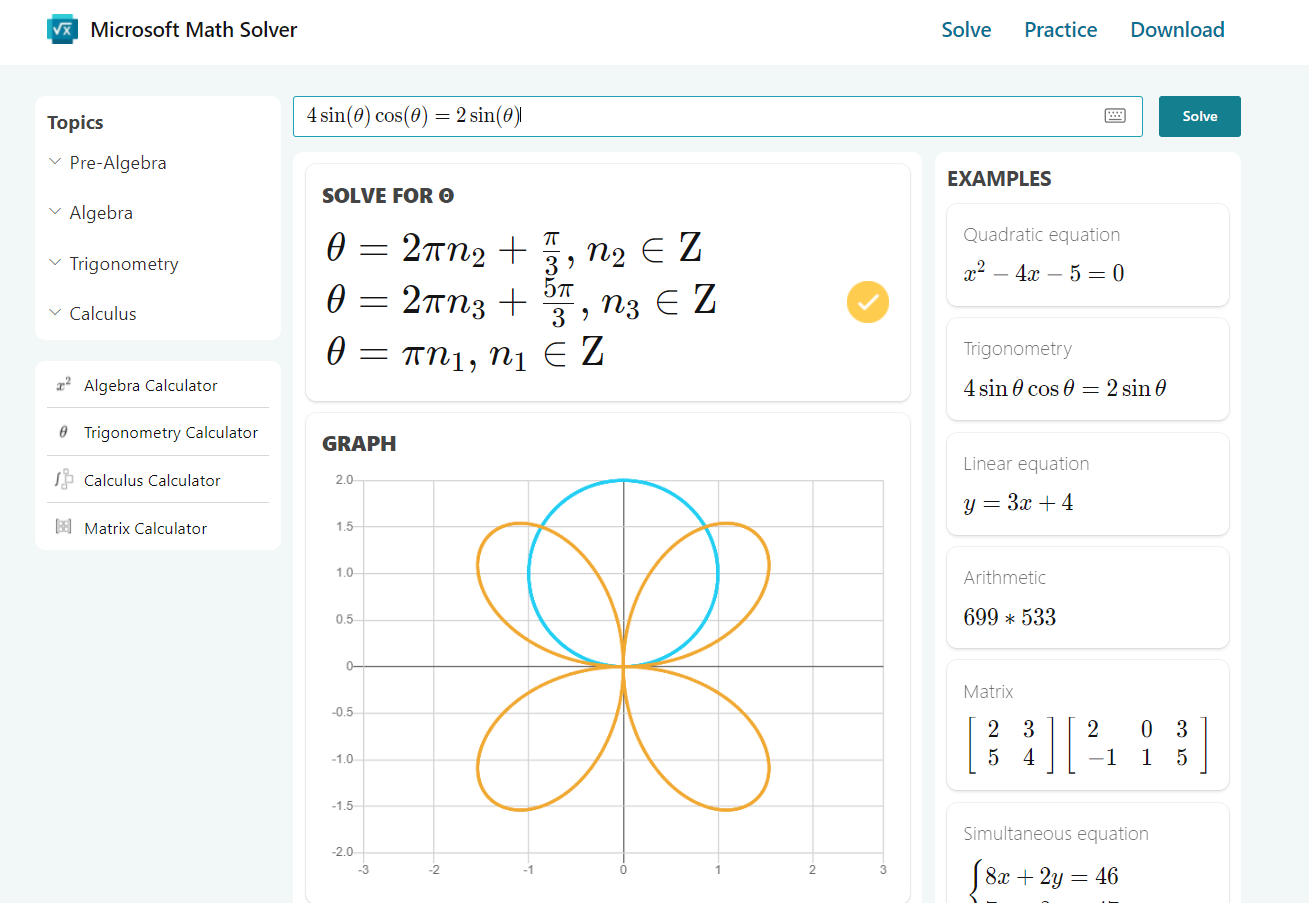
\includegraphics[scale=0.4]{mathsolver3.png}
		\label{fig:output}
	\end{figure}
	\begin{figure}[H]
		\caption{Topics split into sections found in the A-Level Curriculum}
		\centering
		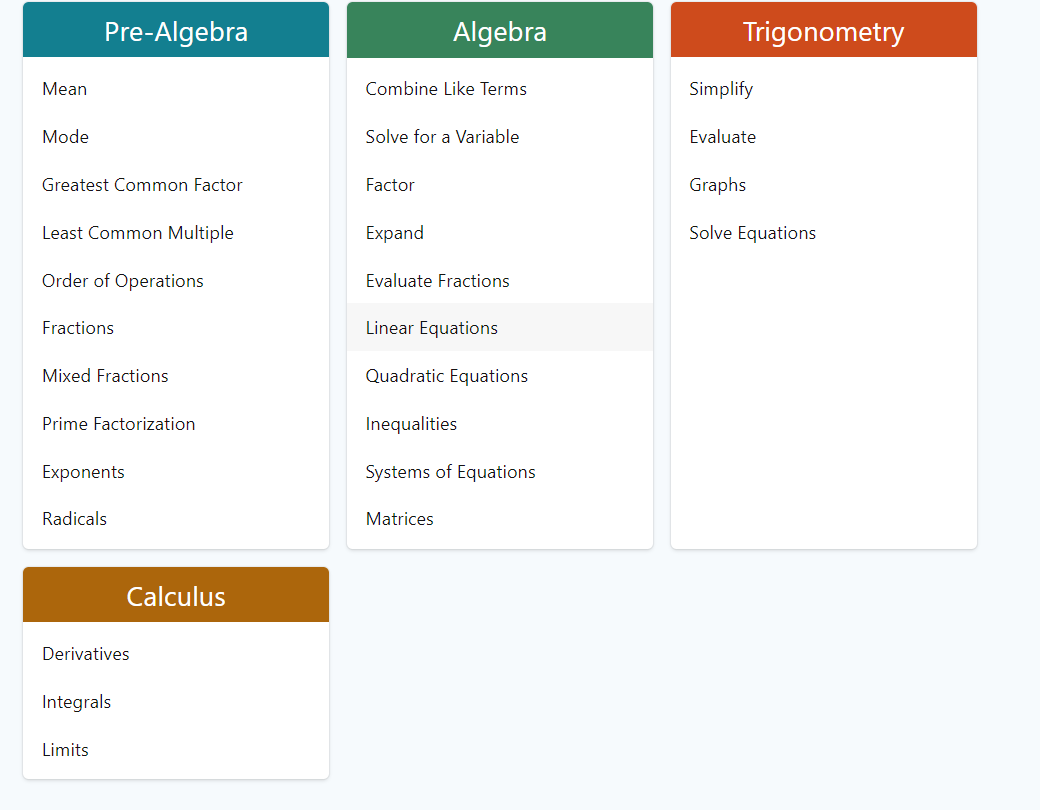
\includegraphics[scale=0.3]{mathsolver2.png}
		\label{fig:topic}
		\end{figure}
	\begin{figure}[H]
		\caption{Calculator Input}
		\centering
		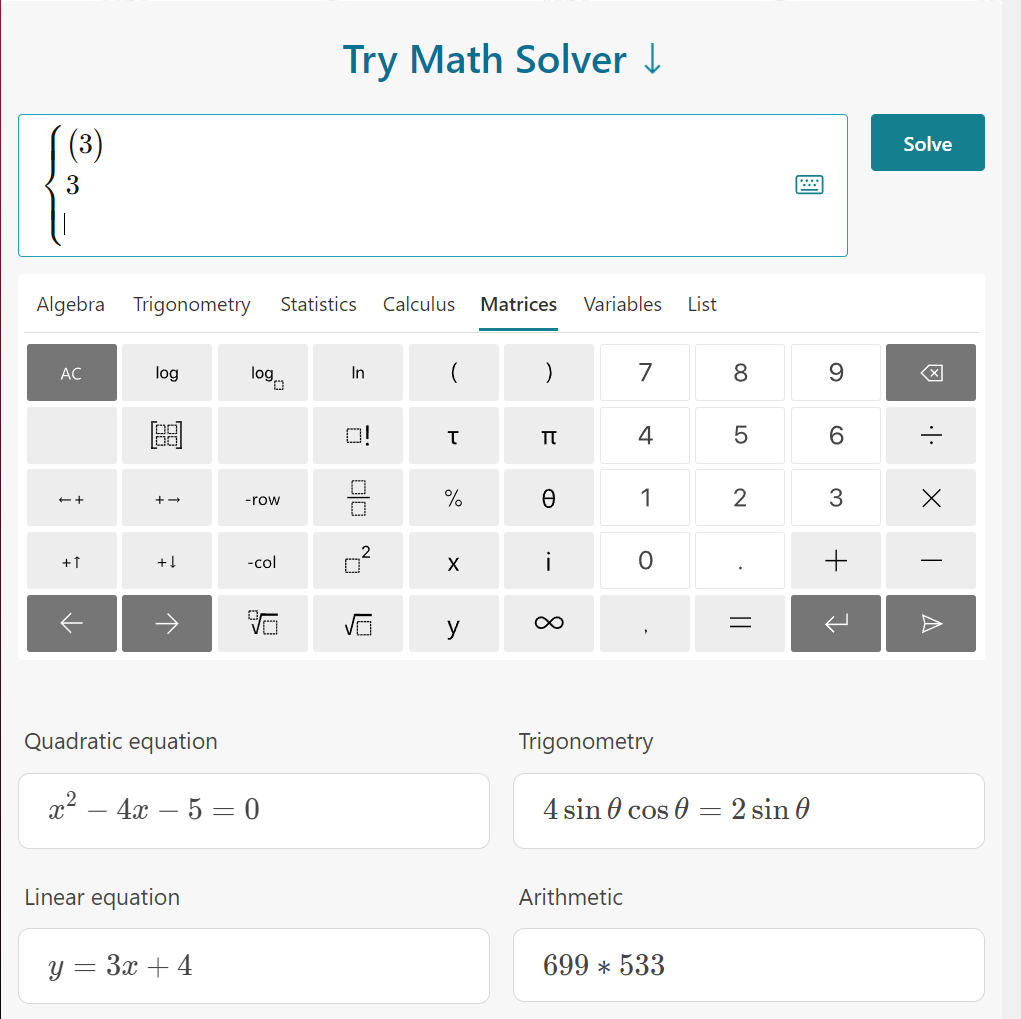
\includegraphics[scale=0.3]{mathsolver.png}
		\label{fig:calc}
	\end{figure}
	
	This source answers the conceptual challenge of which features I do not want the application to hold. The source showed me that step-by-step solutions should be a requirement for parts of my application, as my target audience will need to know how the solution was obtained. I have not used the layout of categories shown in Figure \ref{fig:topic}.I concluded that a calculator input style is not needed for my application and will only be implemented, like in Figure \ref{fig:calc}, if there is enough time left at the end of the development stage.
	
	\subsection{Revision Maths} \label{sec:rev}
	
	Revision Maths is a website that provides GCSE and A-Level revision materials for mathematics. \citet{revision}. This source will be used to decide which topics of mathematics I need to include, from reviewing it's difficulty. This is because usually students will need to get solutions on the more complex topics, making them a priority to include in my project. Based on the pages the source provided me (in Calculus and Algebra sections), I concluded that my application will need to address differentiation and integration problems as a priority.\\
	\\This helped in my class design (\ref{sec:class} when choosing topics for calculus such as differentiation and integration. This source was also used to learn and create algorithms to solve problems involving vectors. Figure \ref{fig:rev} is the vectors page for A-Level students. It shows two categories that will be in the vectors part of my application named "Vector Equation of a Line" and "Scalar Product". Using information such as representing line equations, will help to understand what the user needs to input. The example under "Vector Equation of a Line" then shows myself how I can solve the problem, but the fact there is only one example means the source is not highly effective for education. Furthermore dimension of vectors in the example is two whereas it is usually three for A-Level students.\\

		\begin{figure}[H]
		\caption{Information on the page regarding vectors, showing how to find the point of intersection of two lines, and finding the scalar product}
		\centering
		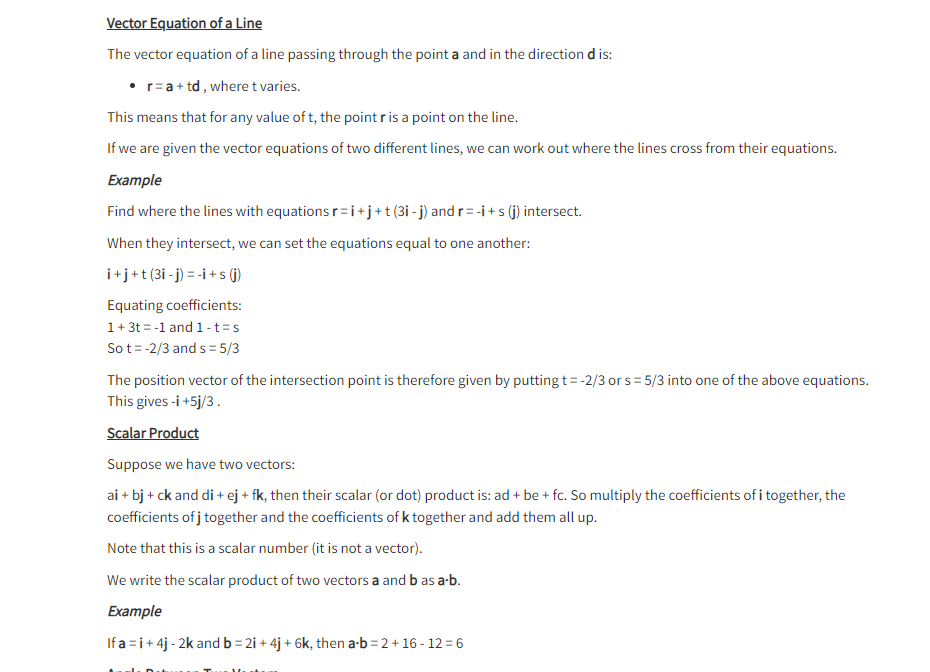
\includegraphics[scale=0.6]{revisionmaths.png}
		\label{fig:rev}
	\end{figure}
	Revision Maths (\cite{revision}) will not be used as frequently as other sources because it fails to contain information regarding other important topics, such as Matrices. Furthermore, the source is very brief on each topic which will not aid hugely in designing algorithms.
	
	\subsection{Further Maths Tutor} \label{sec:fur}
	
	Further Maths Tutor is similar to the source in subsection \ref{sec:rev} but provides revision materials for A-Level Further Mathematics. \cite{furthermaths}. This will aid in understanding the mathematical problems at hand, and what to typically expect a student will want to know. \\
	\\Figure \ref{fig:further} shows the simultaneous equations section on the matrices page. It shows how to solve a system of equations using matrix coefficients. Below that it then described how to get the solution by inverting the matrix to get the results. All these matrix operations will be in my application. The page also gives examples to further explain the issue. 
	
		\begin{figure}[H]
		\caption{Further Maths Tutor - FP1 Matrices page on simultaneous equations}
		\centering
		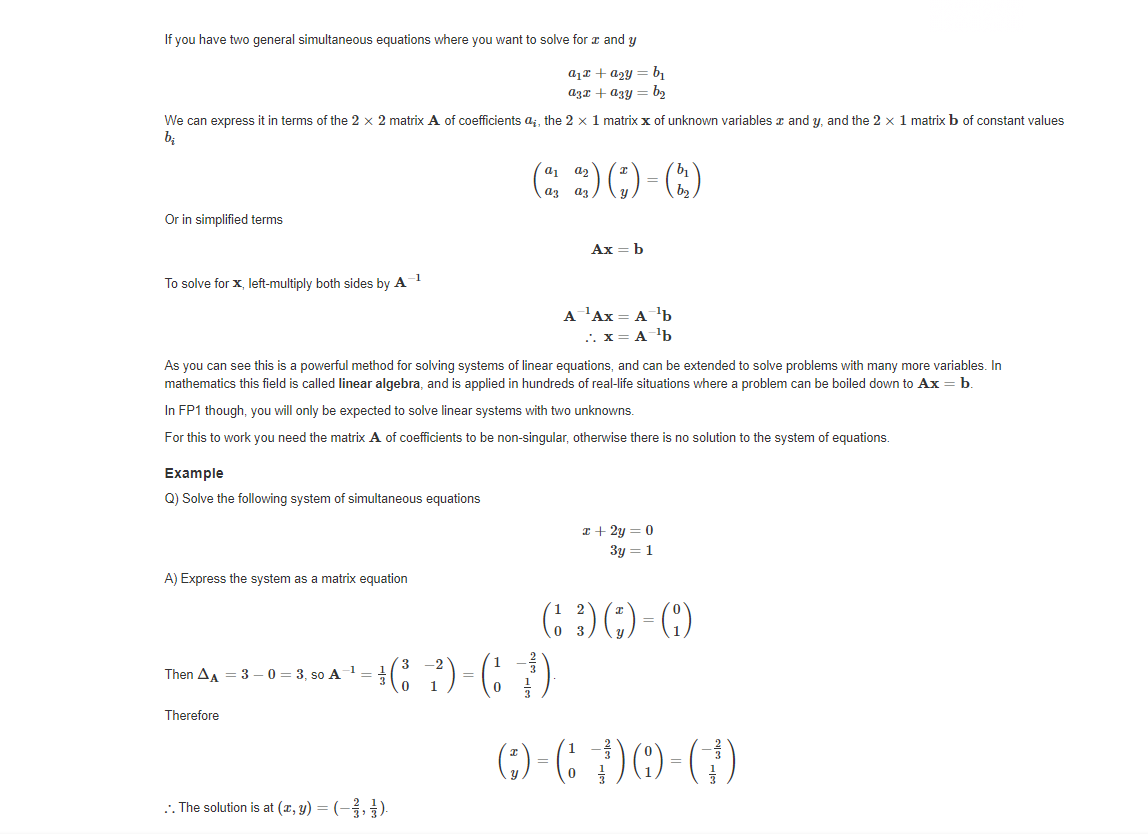
\includegraphics[scale=0.6]{furthermaths.png}
		\label{fig:further}
	\end{figure}
	
	This source will be used extensively for designing algorithms involving matrices and linear equations. It also helps to pick what topics to have in my application, as the topics will be ones students will usually use. 
	
	\subsection{PySimpleGUI Documentation} \label{sec:pysimple}
	
	PySimpleGUI is the graphical interface library that is being used for this project. To decide what library would be best to use, that achieves all the goals of the project, I used PySimpleGUI's official documentation. \cite{py}.\\
	\\The documentation provides demo programs, which allowed me to quickly see what my GUI could look like. An example of a demo program is in Figure \ref{fig:demo}, this is the "All Elements" demo which displays most features the GUI can do in a few windows. The figure shows a custom title bar, followed by a top-menu, and then pages containing different elements. Elements displayed on the figure consist of buttons, input boxes and pop-ups.
	\begin{figure}[H]
		\caption{Demo Program - All Elements}
		\centering
		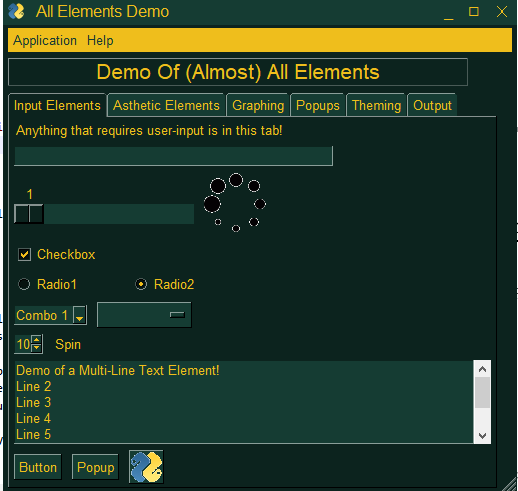
\includegraphics[scale=0.6]{demoprogram.png}
		\label{fig:demo}
	\end{figure}
	The code in the program seemed very simple and easy to use, due to the fact elements and parameters were named appropriately e.g. creating a button was as simple as listing the library followed by the object "Button". The button then had many parameters listed as "size" and "text".\\ 
	\\Within the documentation, I could research every element and get a detailed explanation on what the element does, and what it's parameters can do. Take button images as an example in Figure \ref{fig:button}, which shows the documentation on the element. You can clearly see the figure gives a brief description of the requirements of using the elements. "Your button images need to be in PNG or GIF format." \cite{py}. Then on the bottom two white boxes, it details the parameters and gives a brief description about them. 
		\begin{figure}[H]
		\caption{Documentation on Button Images}
		\centering
		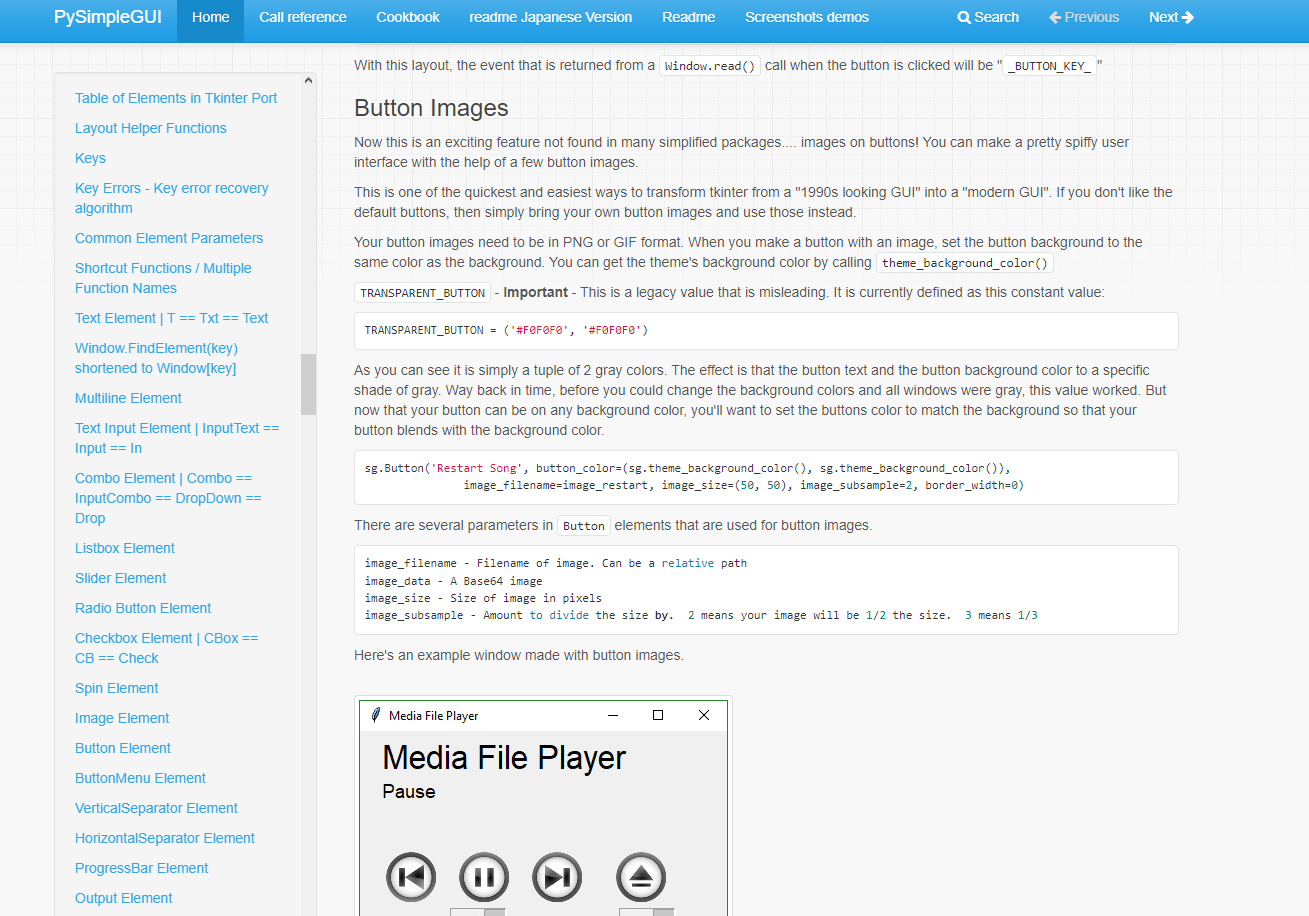
\includegraphics[scale=0.5]{buttonimg.png}
		\label{fig:button}
	\end{figure}


	\section{Methodology}\label{sec:method}
	
	In this section I will detail how I produced the results in \ref{sec:results}. This will be explained through my class design, testing, planning and programming. Each section should contribute to answering any questions or issues encountered in the introduction \ref{sec:intro} and Literature review \ref{sec:lit}.
	
	\subsection{Class Design} \label{sec:class} 
	
	This section will detail the application's class design and it's benefits.\\
	\\The classes are split into two separate directories, one folder contains the test files and the other holds application files. These are split into 5 separate files as can be seen in my Class diagram in Figure \ref{fig:uml}. This class diagram is what I used to structure my code layout to achieve the results.\\
	\\The Matrices and Vectors class were responsible for handling all matrix and vector operations. Both classes had methods that dealt with creating the correct array structure, given a 1D array. It also has methods to type check all the fields the user has inputted such as $typeCheck$ in the vectors class. Methods that deal with simultaneous equations are found in the Matrices class as the solution involves matrices only.\\
	\\The class GUI holds methods only involving the GUI aside from $createStringResult$. Variables are held containing objects to each other file, allowing access to the operations received from the GUI.\\
	\\Layout was not in my original class design, but was added to make the class GUI more readable and easier to develop with. This was due to the GUI class being far too long due to having so many methods, making the editing a lot harder. The Layout class contains all methods for creating the window on each page. It also holds variables for image data on the buttons. \\
	\\Each file will have a test file, which is written as the class is developed. A large part of content for the tests is found in the "testMatrices" and "testVectors" boxes.\\
	\\Having predefined methods to work from gives a very good basis on beginning development. The edges on each node represents which classes reference each other, giving a very structured outlook on how the application should be made.
	\begin{figure}[H]
		\caption{UML diagram showing the classes and methods I aim to create in code development.}
		\centering
		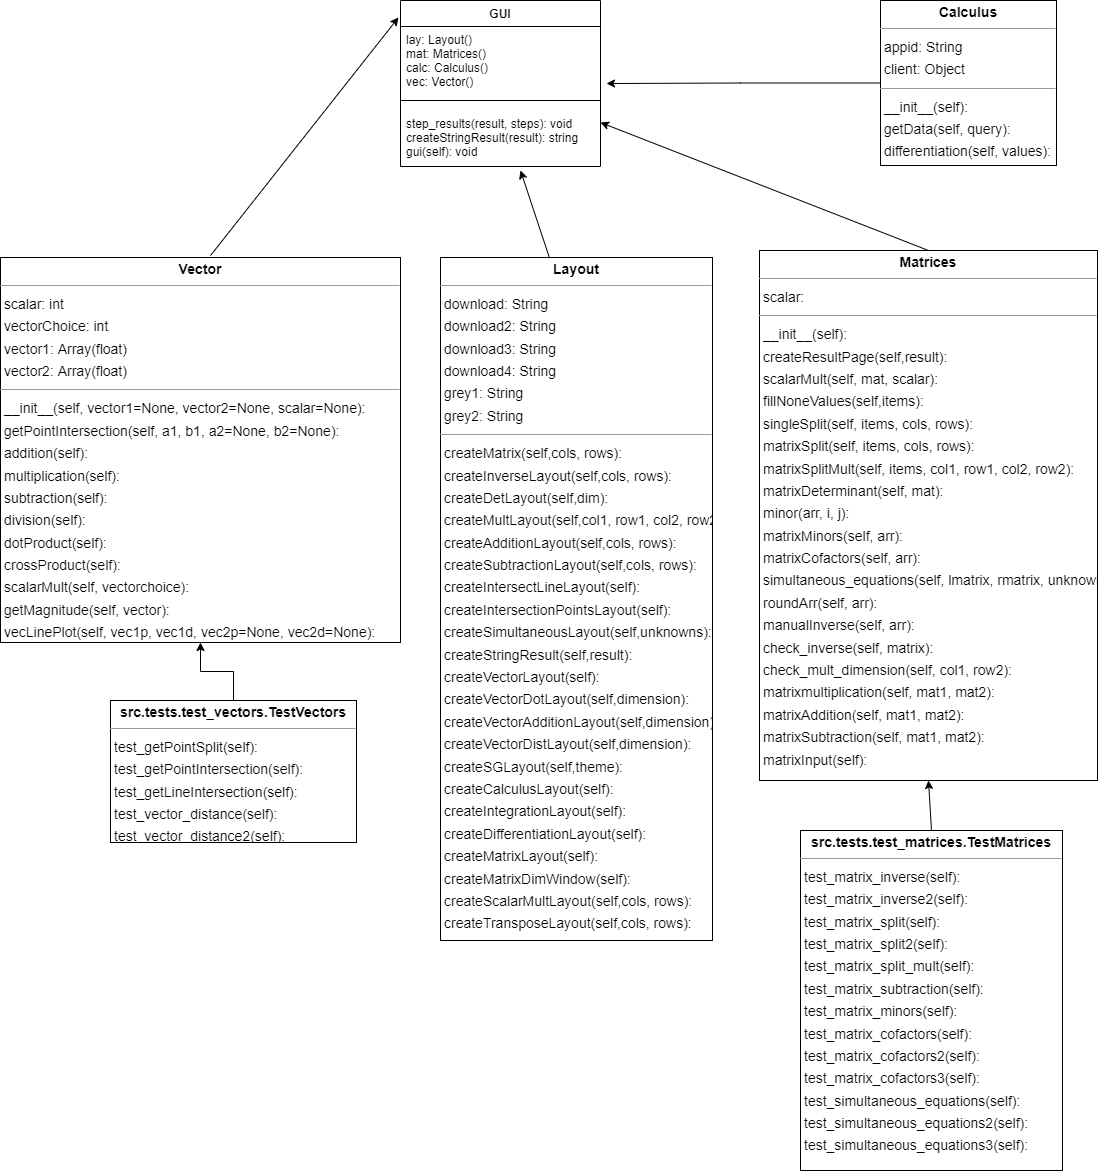
\includegraphics[scale=0.4]{UML.png}
		\label{fig:uml}
	\end{figure}
	\subsection{Planning} \label{sec:planning}
	
	In this section I will describe the project plan and how it's implementation helped produce my results. The plan should be accurate, realistic and account for possible adjustments that may need to be made.\\
	\\I assigned 26 weeks to complete the project from the assignment date. This was based on my experience of designing tests and mathematical operations, and how long each stage would take. I also felt this was an appropriate number of weeks as I expect to have finished the application by week 20, leaving 6 extra weeks.\\
	\\The plan was split into stages to show the final week a section should be completed. It also helped detail the different stages of development, ranging from class to GUI design, and then the development. These stages are then split into subsections, making the plan more concise and accurate. \\
	\\My project plan is represented in Figure \ref{fig:gantt}, which shows all the stages from weeks 1 to 26. A Gantt chart was used to display the length of each task. Stage 1 shows the tasks consist of literature review (as discussed in \ref{sec:lit}), followed by creating a UML diagram which is part of the Class Design \ref{sec:class}. I expect to have completed stage 1 by week 5.\\
		\definecolor{barblue}{RGB}{153,204,254}
	\definecolor{groupblue}{RGB}{51,102,254}
	\definecolor{linkred}{RGB}{165,0,33}
	\renewcommand\sfdefault{phv}
	\renewcommand\mddefault{mc}
	\renewcommand\bfdefault{bc}
	\setganttlinklabel{s-s}{START-TO-START}
	\setganttlinklabel{f-s}{FINISH-TO-START}
	\setganttlinklabel{f-f}{FINISH-TO-FINISH}
	\sffamily
	\begin{figure}[H]
		\label{fig:gantt}
		\caption{Gantt Chart - Project Plan detailing how I will complete my goals from 1-28 weeks.}
		\begin{ganttchart}[
			canvas/.append style={fill=none, draw=black!5, line width=.75pt},
			hgrid style/.style={draw=black!5, line width=.75pt},
			vgrid={*1{draw=black!5, line width=.75pt}},
			x unit = 0.4cm,
			title/.style={draw=none, fill=none},
			title label font=\bfseries\footnotesize,
			title label node/.append style={below=7pt},
			include title in canvas=false,
			bar label font=\mdseries\small\color{black!70},
			bar label node/.append style={left=2cm},
			bar/.append style={draw=none, fill=blue!63},
			bar incomplete/.append style={fill=barblue},
			bar progress label font=\mdseries\footnotesize\color{black!70},
			group/.append style={draw=none, fill=blue!63},
			group incomplete/.append style={fill=groupblue},
			group left shift=0,
			group right shift=0,
			group height=.5,
			group peaks tip position=0,
			group label node/.append style={left=.6cm},
			group progress label font=\bfseries\small,
			link/.style={-latex, line width=1.5pt, linkred},
			link label font=\scriptsize\bfseries,
			link label node/.append style={below left=-2pt and 0pt}
			]{1}{26}\label{gant}
			\gantttitle[
			title label node/.append style={below left=7pt and -3pt}
			]{WEEKS:\quad1}{1}
			\gantttitlelist{2,...,26}{1} \\
			\ganttgroup{Stage 1}{1}{4} \\
			\ganttbar[
			name=1.1
			]{\textbf{1:} Research on library}{1}{2} \\
			\ganttbar[
			name=1.2
			]{\textbf{2:} Create UML}{2}{4} \\[grid]
			\ganttgroup{Stage 2}{4}{13} \\
			\ganttbar[name=2.1]{\textbf{1:} Matrices}{4}{7} \\
			
			\ganttbar[name=2.3]{\textbf{2:} Vectors}{7}{10} \\
			\ganttbar[name=2.2]{\textbf{3:} Develop tests}{5}{13} \\[grid]
			
			\ganttgroup{Stage 3}{13}{20} \\
			\ganttbar[name=3.1]{\textbf{1:} GUI design}{13}{14} \\
			\ganttbar[name=3.2]{\textbf{2:} GUI development}{15}{19} \\
			\ganttbar[name=3.3]{\textbf{3:} User Testing}{15}{20} \\
			\ganttgroup{Final Stage}{20}{26} \\
			\ganttbar[name=4.1]{\textbf{1:} Code Quality review}{20}{22} \\
			\ganttbar[name=4.1]{\textbf{2:} Extra features}{22}{24} \\
			\ganttbar[name=4.2]{\textbf{2:} Debugging}{20}{26} \\
			
		\end{ganttchart}
		
	\end{figure}

	Stage 2 is development of the back-end part of the application, which is to create and test all classes involving mathematical operations. This stage starts directly after Stage 1, and should be completed by week 13. Stage 3 is then responsible for creating the GUI(graphical user interface), which involves the design and development. User testing should be carried out from the start of production(week 15) to the end of Stage 3(week 20).\\
	\\The final stage has a code quality review from weeks 20 to week 22. This part of the stage should improve code on the basic application produced from the previous stages. This is then followed by accounting for any errors in debugging and adding extra features that are not detailed in the plan.\\
	\\As mentioned earlier, the application should have been finished by week 20 so the final stage is only applicable if the plan has been met on time. Debugging and extra features are not a necessary part of the plan, as any errors should be fixed in the development stage by the class and user testing. Any extra features are optional and don't add to the goal of the project.\\
	The plan accounted for time issues by giving 6 extra weeks in the case of unforeseen circumstances making it more achievable. By mitigating any errors in development by enforcing regular testing, the chances of unforeseen circumstances hugely decrease meaning the plan becomes more accurate. Finally, the categorising of different stages made the plan concise, meeting all the goals for a project plan.

	
	\subsection{Code Development}
	
	This section will describe how I developed my application with the Python language. I will touch on all the classes mentioned in Section \ref{sec:class}. I used the PyCharm Professional IDE (Integrated Development Enviroment) for all code development. I chose this IDE due to having features such as code coverage monitoring and debugging.\\
	\\For most vector and matrix operations, I used the 'Numpy' library. This is imported in each class as 'np'. The library allows arrays to be stored as vectors or matrices, and then stores a large collection of mathematical functions to operate on those arrays. For example, in Figure \ref{fig:numpy} there are 5 definitions which contain operations such as addition, multiplication, subtraction and determinants.\\ 
	\\The definition $matrixMultiplication()$ in Figure \ref{fig:numpy} makes use of the multiplication operation by using $np.dot$ which means to find the dot product of the two arrays provided. To help describe what that operation is doing, I created an algorithm which would return the identical result to $np.dot$. This can be found at Algorithm \ref{alg:alg0}.
	
	\begin{figure}[H]
		\caption{Use of Numpy operations in matrices.py}
		\centering
		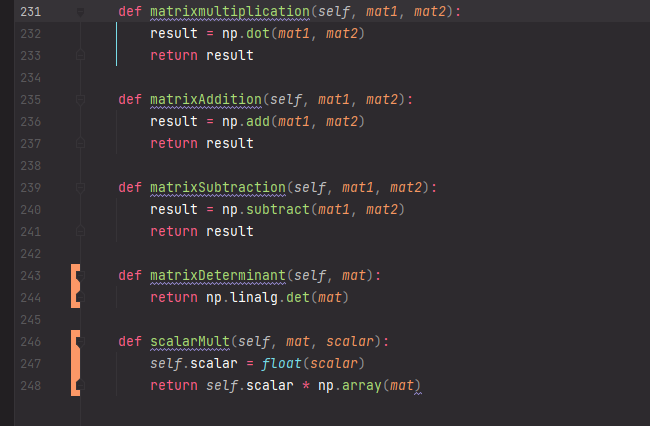
\includegraphics[scale=0.7]{numpy.png}
		\label{fig:numpy}
	\end{figure}

	\begin{algorithm}
	\caption{Matrix multiplication}\label{alg:alg0}
	\begin{algorithmic}[0]
		
		\Procedure{multiplyMatrix}{$a,b$}  
		\State $result \Leftarrow matrix[$length $a, $length $a +1] $
		\For {i in length $a}$
		\For{j in length $b[0]}$
		\For{k in length $b}$
		\State $result[i][j] \Leftarrow result[i][j] + a[i][k]*b[k][j]$
		\EndFor
		\EndFor
		\EndFor
		\Return $result$
		\EndProcedure
	\end{algorithmic}
\end{algorithm}
	To create the Matrices class, I needed methods to split up 1-D arrays into multiple dimensional arrays. This will allow them to be represented as matrices so they can be operated on by the Numpy library. The GUI will send a long list of values to these methods that should be split up based on the number of columns and rows. To do this I created three methods based on three different circumstances the user will input. The method $singleSplit(arr, cols, rows)$ accounts for the user inputting one matrix, $matrixSplit(items, cols, rows)$ accounts for the user inputting two matrices and the method $matrixSplitMult(items, col1, row1, col2)$ handles a user inputting two matrices of different dimensions.\\
	\\An algorithm was designed for splitting matrices and vectors into the correct dimensional arrays. Algorithm \ref{alg:Algorithm1} shows how a 1-Dimensional array can be split into an array with dimensions according to the columns and rows. This algorithm is then used to create the definition in Figure \ref{fig:single} which shows a single definition in matrices.py named $singleSplit(arr, cols, rows)$. By designing these algorithms, it saved me a lot of time while coding as I had predefined solutions to my problem, which in this case was getting the values from the GUI and into arrays that can be operated on.\\
	\\
	\begin{algorithm}
		\caption{Matrix Split}\label{alg:Algorithm1}
		\begin{algorithmic}[1]
			
			\Procedure{singleSplit}{$arr,columns, rows$}  
			\State $result \Leftarrow [ ] $
			\State $i \Leftarrow 0 $
			\State $arrpos \Leftarrow 1 $
			\State $currentArr \Leftarrow [ ] $
			\For {$x$ in $arr$}
			\If{$i < (columns * rows$)}
			\State $num \Leftarrow x$
			\State $currentArr \Leftarrow currentArr + num$
			\If{$arrpos = columns$}
			\State $result \Leftarrow result + currentArr$
			\State $currentArr \Leftarrow [ ] $
			\State $arrpos \Leftarrow 1 $
			\Else
			\State $arrpos \Leftarrow arrpos + 1 $
			\EndIf
			\EndIf
			\EndFor
			\Return $result$
			\EndProcedure
		\end{algorithmic}
	\end{algorithm}
	\begin{figure}[H]
		\caption{Use of singleSplit algorithm in matrices.py}
		\centering
		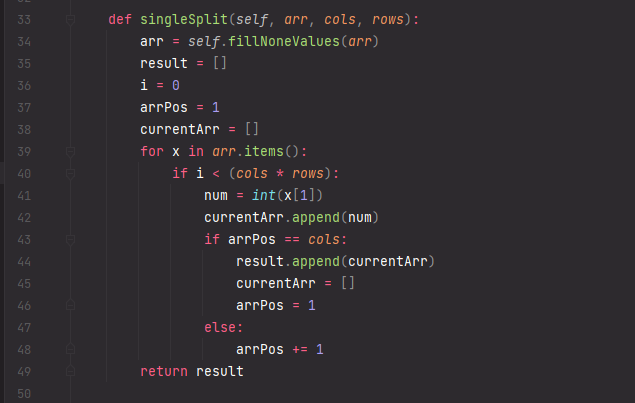
\includegraphics[scale=0.7]{singlesplit.png}
		\label{fig:single}
	\end{figure}
	The rest of the class is responsible for handling operations using the 'Numpy' library and contains methods to return results the user can read. The method named $truncate(n, decimals=0)$ will round an array based on the number of decimals provided. I used Algorithm \ref{alg:round} to create the method. This definition is needed as the resulting matrix could have recurring values which means the user would find it very hard to read the result if it is too long. 	
	\begin{algorithm}
		\caption{Rounding a Matrix Algorithm used to create the 'truncate' definition}\label{alg:round}
		\begin{algorithmic}[3]
			\Procedure{RoundArr}{$arr,d$}
			\State $multiplier \Leftarrow 10^d$
			\State $arr \Leftarrow matrix[n>=1][n>=1]$
			\For {i in $arr[0]$}
			\For {j in $arr[1]$}
			\State $arr[i][j] \Leftarrow (arr[i][j]*multiplier)/multiplier$
			\EndFor
			\EndFor
			\Return $arr$
			\EndProcedure			
		\end{algorithmic}
	\end{algorithm}

	The Matrices and Vector class are very similar in terms of the operations it uses and executes. However, the methods for splitting the items received by the user are done manually in the Vector class, by setting predefined keys in the "layouts.py" file. Figure \ref{fig:vecsplit} shows a definition called $getVecOpItems()$. This definition takes in the user input and assigns vector variables depending on the keys in the values dictionary. The dictionary $values$ is passed into the method and contains all information regarding the GUI, such as user inputs. The reason predefined values had to be set beforehand is because the vectors have certain dimensions that need to be split accordingly (e.g. line intersection requires 4 different vectors).
	
		\begin{figure}[H]
		\caption{Definition in vectors.py, showing user input being split into a vector through key checking}
		\centering
		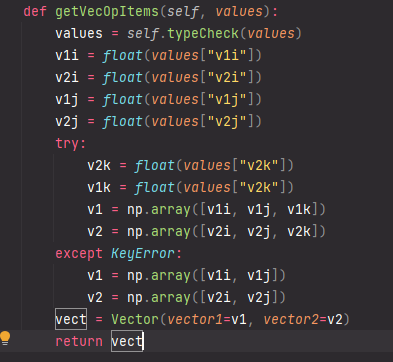
\includegraphics[scale=0.7]{vectorkey.png}
		\label{fig:vecsplit}
	\end{figure}
	
	The file "layouts.py" contains a class called Layout. This class holds image data, definitions to create buttons and layouts and further methods to avoid repeated code. Image data would be held in string variables for buttons and icons. This allowed the GUI to have modern and more presentable buttons, improving the 'feel' of the application.\\
	\\Each window created in the GUI, each has a designated method in the Layouts class. For example, the vectors page (page shown after "Vectors" is pressed from the home screen) is created through the definition shown in Figure \ref{fig:veclayout}. What the definition contains is an array called "vectorLayout" holding elements to be displayed on the window. The first element is a call to the top layer of the application, through another method called $createTopLayer()$. The top layer can be seen on all pages and holds the title along with a help and home button. The next items in the array contain labelled frames (boxes to hold elements), buttons for the user to select operations and selection boxes for the user to specify dimensions for the operation. Finally, the definition returns a "Window" holding the title, layout of the application ($vectorLayout$), size and further possible options such as 'resizable'. This is generally how each definition in the Layouts class will create windows to be displayed to the user.  

	\begin{figure}[H]
		\caption{Definition in vectors.py, showing how the Vectors window is created}
		\centering
		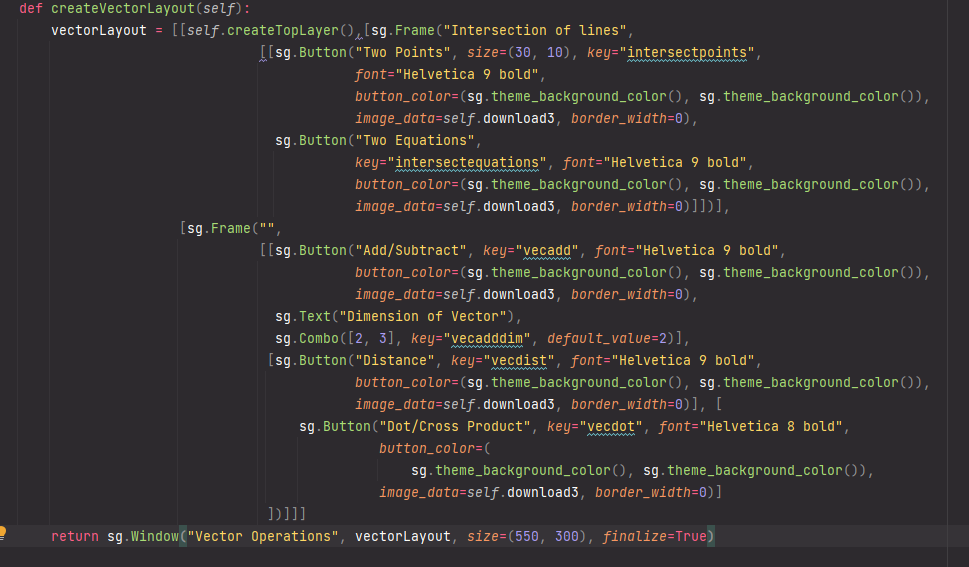
\includegraphics[scale=0.7]{veclayout.png}
		\label{fig:veclayout}
	\end{figure}
	Repeated code in the file "layouts.py" was avoided by having definitions such as $createMatrix(self, cols, rows)$ which returns an array containing the layout of a matrix based on the columns and rows specified in the parameter. This method was used in every window containing matrices.
	
	\section{Results} \label{sec:results}
	
	In this section I will be detailing the results obtained through the methodology. The main result in the final program will be the GUI (Graphical User Interface) in which the client will be using. Upon using this GUI, users can carry out mathematical operations and receive a result verifying if their answer is correct. I have used the Matrices section of my application to detail features that can be expected from every other section.\\
	
	\subsection{GUI} \label{sec:gui}
	
	In this section I will layout the main feature of the application, the GUI(Graphical User Interface). This is the default way the user will access the software.\\
	\\Upon launching the program, a GUI will appear at the starting screen titled "Home". The home page of the program can be seen in Figure \ref{fig:GUI}. The top layer of the program contains the title (StudentSolver) at the centre, a home button to the left and a help button to the right. Underneath this is a text input box where the user can input any question mathematics related and receive the correct answer after pressing the solve button. \\
	\\Below this are further options. The options for the user to select are simple and categorised for maths students. The choice of Vectors, Matrices and Calculus can be seen in the frame, and a simultaneous equations button with a list box option to choose the number of unknowns.\\
	\\A further feature is added for selecting the program's theme which is a feature no other mathematical applications have. Being able to choose a colour scheme can be important to students, as colour schemes can grab attention and also make text easier to read on the GUI. \\

	
	\begin{figure}[H]
		\caption{Home page displayed to the user upon launching the application. Contains home button, help button, question boxes and buttons for navigation.}
		\centering
		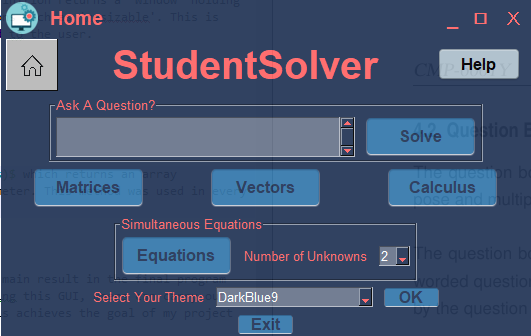
\includegraphics[scale=1]{GUI.png}
		\label{fig:GUI}
	\end{figure}
	
	\subsection{Question Box} \label{sec:question}
	
	The question box was briefly mentioned in \ref{sec:gui}, this section will explain further it's purpose and multiple uses.\\
	\\The question box can be seen in figure \ref{fig:GUI} as an input box within the frame labelled "Ask a Question", and It's purpose is for the user to input any worded question to get a result. Every other operation in the program can also be done by the question box.\\
	\\For example, say the user wanted to get the dot product of two vectors, they can simply input "dot product (1,2,3),(1,2,2)". The input and result can be seen in Figure \ref{fig:question}. The output clearly shows that the result is 11. The question box will also adjust to small syntax errors the user can make such as spacing or capitals. If the user inputted "dOt product   (1,2  ,3),(1,2 , 2)", the result would be the same. This is especially helpful for students that might not be aware of mathematical syntax, which most students are not.\\
	\\Not only can this feature do everything the program can do, it can solve questions to topics not featured on the application. If the user was to input "plot 2x" a window is created with the plotted data on a graph as shown in Figure *. Simple equations can be solved through this feature as mentioned by the help button. The user inputting "solve 2x+5=4" will yield a result of "x=-0.5".\\
	\\In cases where there are no results, the output box will display "No results!". This will only occur when there is no solution to the question asked.  
	
		\begin{figure}[H]
		\caption{Pop-up of results gained from entering "dot product (1,2,3),(1,2,2)" in the question box behind the pop-up}
		\centering
		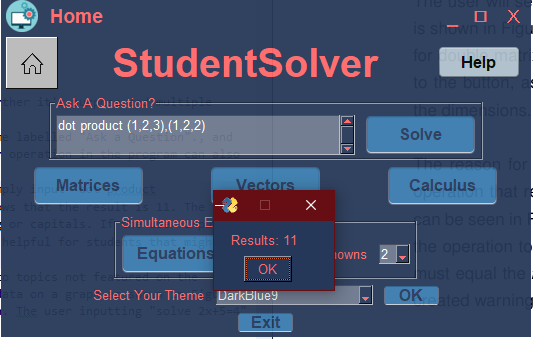
\includegraphics[scale=1]{question.png}
		\label{fig:question}
	\end{figure}
	
	\subsection{Matrices} \label{sec:matrices}
	
	In this section I will explain the resulting action of the user pressing on the button labelled "Matrices" in Figure \ref{fig:GUI}.\\
	\\The user will see a variety of matrix operations to carry out on the Matrices page. This is shown in Figure \ref{fig:matrices}. There are 2 frames, one for single matrix operations and the other for double matrix operations. For each operation, the dimensions can be selected next to the button, aside from matrix multiplication which has a separate page for selecting the dimensions. \\
	\\The reason for this is to make it less complicated for the student, as this is the only operation that requires two matrices of two different dimensions. The selection screen can be seen in Figure \ref{fig:dimensions} For Matrix Multiplication, the dimensions have to be specific for the operation to work. If both matrices are of dimension $m * n$, the $m$ of the first matrix must equal the $n$ of the second matrix. If this condition is not met, a pop-up window is created warning the user.
	
	\begin{figure}[H]
		\caption{Window displayed upon pressing "Matrices" on the home page}
		\centering
		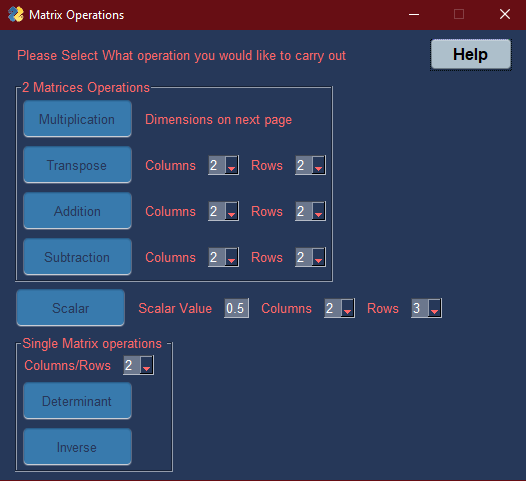
\includegraphics[scale=1]{matrices.png}
		\label{fig:matrices}
	\end{figure}
	\begin{figure}[H]
	\caption{Dimension selection window upon a user pressing "Matrices Multiplication" on the "Matrices" page. 4 Input boxes to select the dimensions of two different matrices}
	\centering
	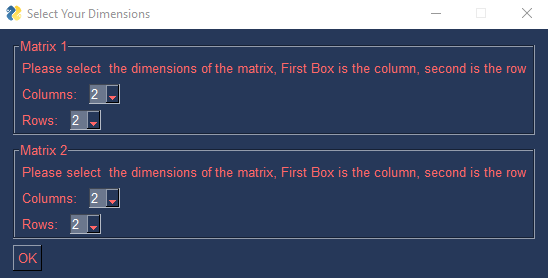
\includegraphics[scale=1]{dim.png}
	\label{fig:dimensions}
	\end{figure}
	
	\subsection{Matrix Inverse} \label{sec:inv}
	
	In this subsection I will detail the action of pressing on the button in Figure \ref{fig:matrices}, labelled Matrix Inverse. The way this page is displayed will have a similar layout to every other operation. Each window involving an operation will contain an output box to display a result, as well as a pop-up upon the user pressing a "Solve" button.\\
	\\An example of a matrix operation that has a feature other programs do not have is detailing the solution step-by-step. This will tell the user each step carried out in the operation, which is especially helpful for inverting a matrix as there are several steps that involve other operations on the matrix screen.\\
	\\As can be seen in Figure \ref{fig:inv}, to input the matrix a set of boxes are laid out and the user is free to input decimals or a whole number. The help button will also notify the user they can press the TAB button in order to quickly input data without the need for mouse movement. This aids the user to navigating around the application, therefore increasing usability. Upon pressing the "Solve" button the user is then told the steps in the output box below. The first step displayed is to find the determinant  of a matrix and inform the user of it. Then the matrix of minors is calculated, followed by applying the matrix of cofactors to it. Then it is transposed, and the result is displayed clearly to the user.\\
	\\This is a very useful feature as all of these operations are in the matrix section of the program, allowing the user to see where they went wrong. However, as not all matrices cannot be inverted, the user will be told why the matrix cannot be inverted and what the determinant is as can be seen in Figure \ref{fig:invnot}.
	
	\begin{figure}[H]
		\caption{Pop-up displayed upon the user entering [1,3,2,2] in the input boxes. Result displayed as [-0.5, 0.7, 0.5, -0.2]. Box below the input boxes show the step-by-step solution}
		\centering
		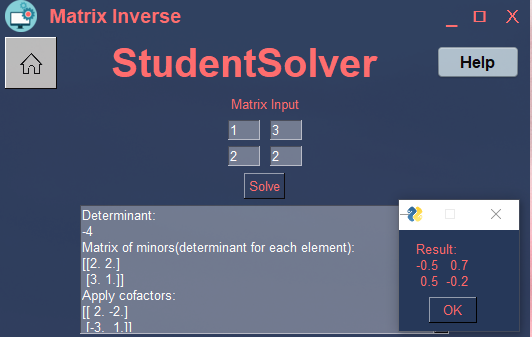
\includegraphics[scale=1]{invert.png}
		\label{fig:inv}
	\end{figure}
	
		\begin{figure}[H]
		\caption{Pop-up displayed upon the user entering [1,1,1,1] in the input boxes. Showing determinant is equal to zero}
		\centering
		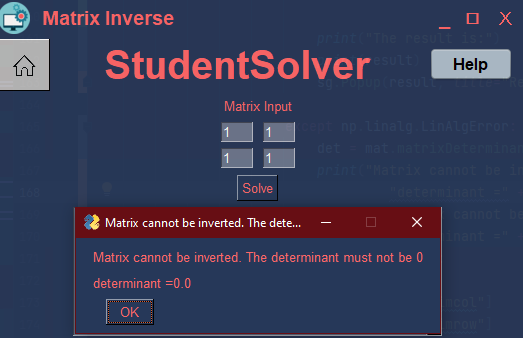
\includegraphics[scale=1]{invertnot.png}
		\label{fig:invnot}
	\end{figure}
	
	
	\subsection{Help Button} \label{sec:help}
	
	Here I will briefly detail the Help button feature and it's uses.\\
	\\The help button creates a pop-up to aid the user in the usability of program and answer any questions the user may have. It can also offer tips such as pressing TAB for faster input and examples of what can be entered into the input box on the home page.\\
	\\As discussed in \ref{sec:gui} and Figure \ref{fig:GUI}, the home page has a help button which offers support on the options the page offers. Other windows will have different results when the user presses the home button. This will help the user with any questions they have on inputting their data, and where they can expect to see the result.\\
	\\Figure \ref{fig:helpbutton} shows the resulting window displayed when the user presses the "Help" button on the home window. It describes how the user should enter a problem in the "Question Box" \ref{sec:question} and information on theme/simultaneous equation selectors. 
	\begin{figure}[H]
		\caption{Pop-up displayed upon the user pressing the "Help" button on the home window}
		\centering
		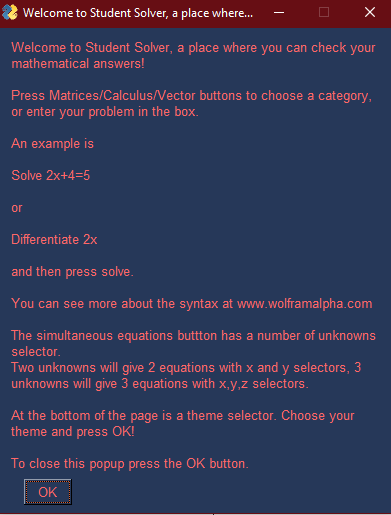
\includegraphics[scale=0.7]{help.png}
		\label{fig:helpbutton}
	\end{figure}
	
	
	\subsection{Testing} \label{sec:test}
	
	In this section I detail the tests that come packaged with the software.\\
	\\Along with the software files, test files can be found in the tests folder. These test the Matrices and Vector operations. Extensive testing is done on the application to ensure there are no errors. The data ranges from alphanumeric to integer/float values.\\
	\\Each function in matrices.py and vectors.py has at least two tests for each function covered, one where an error is expected to be found and one where there is no error. Some features such as simultaneous equations have three tests to check against large data ranges and circumstances where there are no solutions.\\
	\\Testing is an important feature of this program, as it will allow quick debugging for any future work, and high code coverage. Code coverage is the percentage of lines the tests cover in the file it is testing. Figure \ref{fig:coverage} shows my coverage report generated by the tests. It shows the coverage for "vectors.py" is 89 percent, and for "matrices.py" it is 85 percent.
	\begin{figure}[H]
		\caption{Coverage report generated from tests. Shows coverage on the far right column for each file the tests cover.}
		\centering
		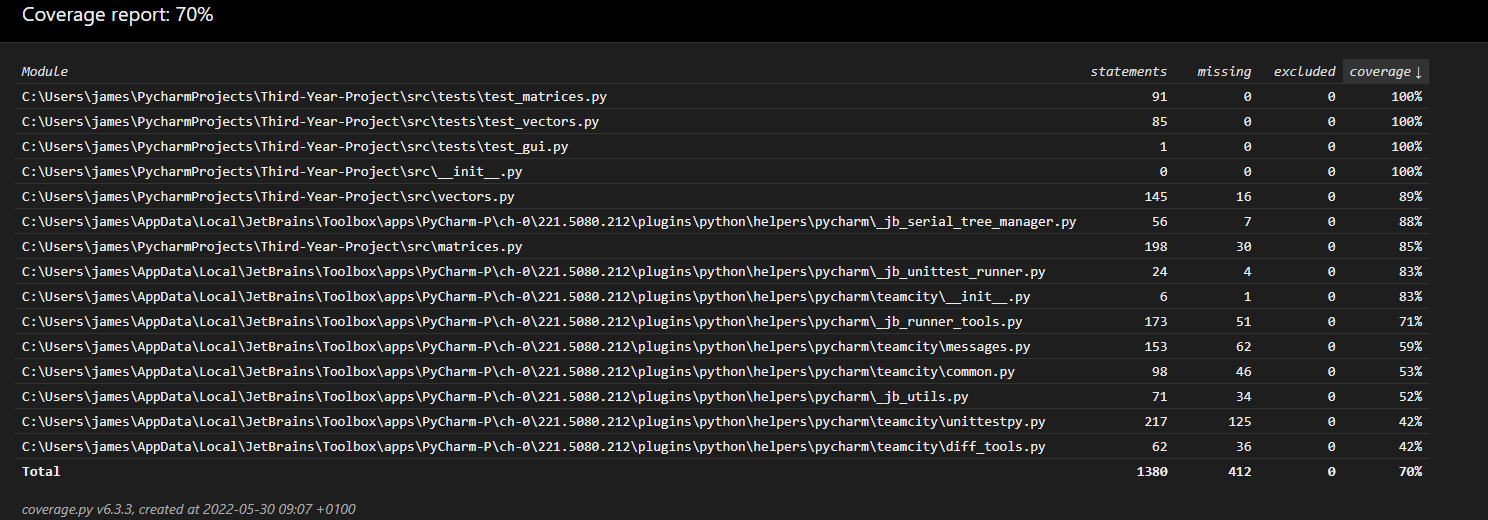
\includegraphics[scale=0.4]{coverage.png}
		\label{fig:coverage}
	\end{figure}
	The report in \ref{fig:coverage} shows there is high code coverage according to business standards. "With that being said it is generally accepted that 80 percent coverage is a good goal to aim for. Trying to reach a higher coverage might turn out to be costly, while not necessary producing enough benefit" \cite{atlassian}. Therefore my application is highly tested according to standards, as both the files the tests cover are above 80 percent.
	

	\section{Conclusion}
	
	The main aim of this project was to develop a working, highly-tested and usable desktop application designed for A-Level Maths students to get correct answers based on the data inputted.\\
	\\The research questions I posed in Section \ref{sec:lit} consisted of what features I want the program to have, how I want the application to look, what mathematical questions need to be answered (and how do I answer them) and what graphical library should I use? Based on the literature review, I decided on features such as a question box and step-by-step solutions. I also decided I did not want features such as calculator inputs in my original plan. How I wanted the application to look was answered more through my GUI design, as opposed to the literature review, so next time I would research some actual desktop applications. \\
	\\The question on what mathematical questions need to be answered were done through research on topics. While it did allow me to decide the questions I want answered in the application, it did not successfully educate me on understanding how to answer the question, meaning I had to rely on usage of the "numpy" library more than I would have liked to. The research on the graphical library in Section \ref{sec:pysimple} aided in creating the GUI and deciding it to be the library of my choice, successfully answering my final research question. The limitations of my research is that there are few programs available aimed at students, meaning design ideas would be hard to retrieve in the form of a desktop application. \\
	\\My methodology section \ref{sec:method} describes how I achieved my results through design, planning and code development. However the lack of user testing through surveying means I developed the program based on my design preference. Despite the application meaning to be simple and have a concise layout, the usability would have definitely benefited by opinions from people who were not involved in development.\\
	\\The results produced, as mentioned in Section \ref{sec:results}, consist of a functional program which has topics on vectors, matrices, calculus and linear equations. The results also produced helping functions and test coverage of over 80 percent. However, I would have also liked to extensively test the Calculus class to improve code coverage in all the classes. \\
	\\In summary, the aims of the project were all met aside from testing. More tests could have been developed if time prevailed and having extensive user testing would have improved the aims of the application being more usable. Therefore, adjusting my plan detailed in \ref{sec:planning} would have allowed more time for proper testing and GUI design.

	\newpage
\newpage
	\bibliographystyle{apalike}
	\bibliography{myBib.bib}
\end{document}
